\documentclass{article}

\usepackage{amsfonts}
\usepackage[fleqn]{amsmath}
\usepackage{mathtools}
\usepackage{stmaryrd}
\usepackage{tikz}
\usepackage{xspace}
\usepackage{xcolor}

\newcommand{\defined}{\ensuremath{\stackrel{\mbox{\tiny def}}{=}}\xspace} %
\newcommand{\vars}{\ensuremath{\mathcal{X}}\xspace} % variables
\newcommand{\vals}{\ensuremath{\mathbb{V}}\xspace} % values
\newcommand{\bvals}{\ensuremath{\mathbb{B}_\mathsf{NA}}\xspace} % bool values
\newcommand{\bools}{\ensuremath{\mathbb{B}}\xspace} % bools
\newcommand{\bna}{\ensuremath{\mathsf{NA}_{B}}\xspace} % bool NA
\newcommand{\ivals}{\ensuremath{\mathbb{Z}_\mathsf{NA}}\xspace} % int values
\newcommand{\ints}{\ensuremath{\mathbb{Z}}\xspace} % ints
\newcommand{\ina}{\ensuremath{\mathsf{NA}_{Z}}\xspace} % int NA
\newcommand{\svals}{\ensuremath{\mathbb{S}_\mathsf{NA}}\xspace} % string values
\newcommand{\strings}{\ensuremath{\mathbb{S}}\xspace} % strings
\newcommand{\sna}{\ensuremath{\mathsf{NA}_{S}}\xspace} % string NA
\newcommand{\isna}{\ensuremath{\mathsf{isNA?}}\xspace} % isNA?
\newcommand{\ipt}{\ensuremath{\mathsf{\mathbf{\color{teal}input}}()}\xspace} % input
\newcommand{\unopexpr}[2]{\ensuremath{#1~#2}\xspace} % unary op expr
\newcommand{\binopexpr}[3]{\ensuremath{#2 #1 #3}\xspace} % binary op expr
\newcommand{\assignstmt}[2]{\ensuremath{#1 := #2}\xspace} % assignment statement
\newcommand{\ifstmt}[3]{\ensuremath{\mathsf{\mathbf{if}}~#1~\mathsf{\mathbf{then}}~#2~\mathsf{\mathbf{else}}~#3~\mathsf{\mathbf{fi}} }\xspace} % if statement
\newcommand{\forstmt}[4]{\ensuremath{\mathsf{\mathbf{for}}~#1~\mathsf{\mathbf{in}}~#2~\mathsf{\mathbf{to}}~#3~\mathsf{\mathbf{do}}~#4~\mathsf{\mathbf{od}}}\xspace} % for statement
\newcommand{\powerset}[1]{\ensuremath{\mathcal{P}\left(#1\right)}\xspace} % powerset
\newcommand{\set}[1]{\ensuremath{\left\{#1\right\}}\xspace} % set
\newcommand{\tuple}[2]{\ensuremath{\langle #1, #2 \rangle}\xspace} % tuple
\newcommand{\lfp}{\ensuremath{\mathrm{lfp}}\xspace} % least fixpoint
%
\newcommand{\labels}{\ensuremath{\mathcal{L}}\xspace} % labels
\newcommand{\envs}{\ensuremath{\mathcal{E}}\xspace} % environments
\newcommand{\files}{\ensuremath{\mathcal{D}}\xspace} % files
\newcommand{\semantics}[1]{\ensuremath{\left\llbracket #1 \right\rrbracket}\xspace} % semantics
\newcommand{\arith}[1]{\ensuremath{\mathcal{A}\semantics{#1}}\xspace} % arithmetic semantics
\newcommand{\bool}[1]{\ensuremath{\mathcal{B}\semantics{#1}}\xspace} % boolean semantics
\newcommand{\stmt}[1]{\ensuremath{\mathcal{S}\semantics{#1}}\xspace} % statement semantics
% dependency semantics
\newcommand{\sdeps}[1]{\ensuremath{\textsc{s-deps}\!\semantics{#1}}\xspace} % static  
\newcommand{\ddeps}[1]{\ensuremath{\textsc{d-deps}\!\semantics{#1}}\xspace} % dynamic
\newcommand{\ids}[1]{\ensuremath{\textsc{vars}\!\semantics{#1}}\xspace} % 
\newcommand{\peek}[1]{\ensuremath{\textsc{peek}\!\semantics{#1}}\xspace} % 
% not-na semantics
\newcommand{\snna}[1]{\ensuremath{\textsc{s-not-na}\!\semantics{#1}}\xspace} % static  
\newcommand{\dnna}[1]{\ensuremath{\textsc{d-not-na}\!\semantics{#1}}\xspace} % dynamic

\newcommand{\irem}[3]{{\noindent\textcolor{#1}{\textsf{[#2: 
#3]}}}}
\newcommand{\todo}[1]{\irem{orange}{TODO}{#1}}	
\newcommand{\note}[1]{\irem{magenta}{NOTE}{#1}}	

\begin{document}

\section*{Syntax}

\begin{figure}[t]
	\begin{center}
		\begin{tabular}{lclr}
			$v$ &$\Coloneqq$& $\mathsf{true} ~~\vert~~ \mathsf{false} ~~\vert~~ \bna$ & $\bvals$\\
			&$\vert$& $\cdots ~~\vert~~ -1 ~~\vert~~ 0 ~~\vert~~ 1 ~~\vert~~ \cdots ~~\vert~~ \ina$ & $\ivals$\\
			&$\vert$& $\cdots ~~\vert~~ \sna$ & $\svals$\\
			\\
			$se$ &$\Coloneqq$& $x$ & $x\in \vars$ \\
			&$\vert$& $v$ & $v \in \vals$ \\
			\\
      $e$ &$\Coloneqq$& $\isna(se)$ & \\
			&$\vert$& $\unopexpr{\circ}{se}$& $\circ~\in \set{\neg, +, -}$ \\
			& $\vert$& $\binopexpr{\diamond}{se_1}{se_2}$& $\diamond \in \set{+, -, *, /, \%, <, \leq, =, \neq, >, \geq, \lor, \land}$ \\
			& $\vert$& $se$ & \\
			\\
			$s$ &$\Coloneqq$& $\assignstmt{x}{e}$ & $x \in \vars$ \\
      &$\vert$& $\assignstmt{x}{\,^\ell{}\ipt}$ & $\ell{} \in \labels$ \\
			&$\vert$& \ifstmt{x}{s_1}{s_2} & \\
			&$\vert$& \forstmt{x}{se_1}{se_2}{s} & \\
			&$\vert$& $s_1 ; s_2$ & \\
			&$\vert$& $e$ & \\
			\\
			P & $\Coloneqq$& $s$ &
		\end{tabular}
	\end{center}
	\vspace{-1em}
	\caption{Syntax}\label{fig:syntax}
\end{figure}

Let \vars be a finite set of program variables, and let $\vals\defined\bvals \cup \ivals \cup \svals$ be a set of values partitioned  in sets of boolean ($\bvals \defined \bools \cup \{\bna\} $), integer ($\ivals \defined \ints \cup \{\ina\} $), and string ($\svals \defined \strings \cup \{\sna\} $) values. Each value type admits a special value $\bna$, $\ina$, or $\sna$ representing missing values.
The syntax of programs is defined inductively in Figure~\ref{fig:syntax}.

\section*{Concrete Input-Aware Semantics}

An environment $\rho\colon \vars \rightarrow \vals$ maps each program variable $X \in \vars$ to its value $\rho(X) \in \vals$. Let \envs denote the set of all environments. 

\todo{Patrick Cousot - Abstract Semantic Dependency (SAS 2019)}


\section*{Syntactic Dependencies}

\subsection*{Static Syntactic Dependencies Analysis}

The program dependency semantics $\sdeps{P} \colon \powerset{\vars \times \labels}$ yields an \emph{over-approximation} of the input-output dependencies of the program $P$:
\begin{equation*}
\sdeps{S^\ell{}} \defined \sdeps{S}\emptyset
\end{equation*}
\note{we start the analysis with the empty set of dependencies}
where the statement dependency semantics $\sdeps{S} \colon \powerset{\vars \times \labels} \rightarrow  \powerset{\vars \times \labels}$ updates the input-output dependencies through the program:

%\begin{figure}[t]
	\begin{align*}
	&\sdeps{^\ell{}X := \ipt}R \defined R \setminus \{ \tuple{X}{\ell{}'} \mid \ell{}' \in \labels \} \cup \{ \tuple{X}{\ell{}} \} 
	%
	\\
	&\mbox{\note{\ipt expressions introduce new dependencies}} \\
	&\sdeps{^\ell{}X := E}R \defined R \setminus \{ \tuple{X}{\ell{}'} \mid \ell{}' \in \labels \} \cup \{ \tuple{X}{\ell{}'} \mid \exists X'\colon X' \in \ids{E} \land \tuple{X'}{\ell{}'} \in R \} \\
	&\qquad\mbox{where $E \not= \ipt$} \\
	&\mbox{\note{\ids{E} is the set of all program variables appearing in the expression $E$}} \\
%
	&\sdeps{\mathsf{\mathbf{if}}~^\ell{}X~\mathsf{\mathbf{then}}~S_1~\mathsf{\mathbf{else}}~S_2~\mathsf{\mathbf{fi}}}R
	 \defined \sdeps{S_1}R \cup \sdeps{S_2}R \\ 
%
&\sdeps{\mathsf{\mathbf{while}}~^\ell{}X~\mathsf{\mathbf{do}}~S~\mathsf{\mathbf{od}}}R
\defined \lfp~R \cup \sdeps{S}\emptyset  \\
&\todo{Is this ok? We keep all dependencies in R to account for executions that do not enter the loop.} \\
&\todo{We iterate to account for the loop executions. It may be equivalent to do $R \cup \sdeps{S}R$.} \\
%
&\sdeps{S_1; S_2}R \defined \sdeps{S_2} \circ 
\sdeps{S_1}R
	\end{align*}
%\end{figure}

\subsection*{Dynamic Syntactic Dependencies Analysis}

\note{this is the semantics for a single run}

	\begin{align*}
	&\ddeps{^\ell{}X := \ipt}R \defined R \setminus \{ \tuple{X}{\ell{}'} \mid \ell{}' \in \labels \} \cup \{ \tuple{X}{\ell{}} \} 
	%
	\\
	&\ddeps{^\ell{}X := E}R \defined R \setminus \{ \tuple{X}{\ell{}'} \mid \ell{}' \in \labels \} \cup \{ \tuple{X}{\ell{}'} \mid \exists X'\colon X' \in \ids{E} \land \tuple{X'}{\ell{}'} \in R \} \\
	&\qquad\mbox{where $E \not= \ipt$} \\
	&\mbox{\note{same as \sdeps{S} so far}} \\
%
	&\ddeps{\mathsf{\mathbf{if}}~^\ell{}X~\mathsf{\mathbf{then}}~S_1~\mathsf{\mathbf{else}}~S_2~\mathsf{\mathbf{fi}}}R
	 \defined \begin{cases} \ddeps{S_1}R & \peek{X} \\
	  \ddeps{S_2}R & \neg \peek{X} \end{cases} \\ 
	  &\mbox{\note{we peek at the actual value of $X$ to choose the execution path}} \\
%
&\ddeps{\mathsf{\mathbf{while}}~^\ell{}X~\mathsf{\mathbf{do}}~S~\mathsf{\mathbf{od}}}R
\defined \begin{cases} \ddeps{\mathsf{\mathbf{while}}~^\ell{}X~\mathsf{\mathbf{do}}~S~\mathsf{\mathbf{od}}} \circ \ddeps{S}R & \peek{X} \\
	  \ddeps{S}R & \neg \peek{X} \end{cases} \\ 
%
&\ddeps{S_1; S_2}R \defined \ddeps{S_2} \circ 
\ddeps{S_1}R
	\end{align*}

\section*{Not-NA Analysis}


	\begin{center}
		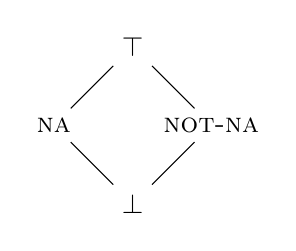
\begin{tikzpicture}[node distance=1cm]
		\node (A) {$\top$};
		\node (B) [below of=A] {};
		\node (C) [left of=B] {\textsc{na}};
		\node (D) [right of=B] {\textsc{not-na}};
		\node (H) [below of=B] {$\bot$};
		\draw (A) -- (C);
		\draw (A) -- (D);
		\draw (C) -- (H);
		\draw (D) -- (H);
		\end{tikzpicture}
	\end{center}
	
\note{We compute dependencies and Not-NA constraints at the same time}
	
\subsection*{Dynamic Not-NA Analysis}


\begin{description}
\item[dependencies] $R \in \powerset{\vars \times \labels}$: pairs of a variable and a program label indicating the label of the input expression the variable depends from;
\item[constraints] $C \in \powerset{\labels}$: program labels of the input expressions that should not be NA; 
\end{description}

\note{this is the semantics for a single run}

	\begin{align*}
	&\dnna{^\ell{}X := \ipt}\tuple{R}{C} \defined \tuple{R'}{C} \\
	&\qquad\mbox{where } R' \defined R \setminus \{ \tuple{X}{\ell{}'} \mid \ell{}' \in \labels \} \cup \{ \tuple{X}{\ell{}} \} 
	%
	\\
	&\ddeps{^\ell{}X := E}\tuple{R}{C} \defined \tuple{R'}{C} \qquad\qquad\qquad\qquad\qquad\qquad\qquad\qquad E \not= \ipt\\
	&\qquad\mbox{where } R' \defined R \setminus \{ \tuple{X}{\ell{}'} \mid \ell{}' \in \labels \} \cup \{ \tuple{X}{\ell{}'} \mid \exists X'\colon X' \in \ids{E} \land \tuple{X'}{\ell{}'} \in R \} \\
%
	&\note{only the dependencies are updated} \\
%
	&\dnna{\mathsf{\mathbf{if}}~^\ell{}X~\mathsf{\mathbf{then}}~S_1~\mathsf{\mathbf{else}}~S_2~\mathsf{\mathbf{fi}}}\tuple{R}{C} \defined \\
	 &\qquad\defined  \begin{cases} \dnna{S_1}\tuple{R}{C'} & \peek{X} \\
	  \dnna{S_2}\tuple{R}{C'} & \neg \peek{X} \end{cases} \\ 
	  &\qquad\mbox{where } C' \defined C \cup \{\ell{}' \in \labels \mid \tuple{X}{\ell{}'} \in R \} \\ 
	  &\note{we update the constraints because $X$ cannot be \textsc{na}} \\
%
&\dnna{\mathsf{\mathbf{while}}~^\ell{}X~\mathsf{\mathbf{do}}~S~\mathsf{\mathbf{od}}} \tuple{R}{C}
\defined \\
&\qquad\defined \begin{cases} \dnna{\mathsf{\mathbf{while}}~^\ell{}X~\mathsf{\mathbf{do}}~S~\mathsf{\mathbf{od}}} \circ \dnna{S}\tuple{R}{C'} & \peek{X} \\
	  \dnna{S}\tuple{R}{C'} & \neg \peek{X} \end{cases} \\ 
	  &\qquad\mbox{where } C' \defined C \cup \{\ell{}' \in \labels \mid \tuple{X}{\ell{}'} \in R \} \\ 
%
&\dnna{S_1; S_2}R \defined \dnna{S_2} \circ 
\dnna{S_1}R
	\end{align*}

\begin{align*}
&^1 a := \ipt \\
&^2 x := \ipt \\
&^3 y := \ipt \\
&^4 b := \textsc{true} \\
& \mathsf{\mathbf{while}}~^5b~\mathsf{\mathbf{do}} \\
& \qquad\mathsf{\mathbf{if}}~^6x == 3~\mathsf{\mathbf{then}} \\
&\qquad\qquad ^7 y = a \\
& \qquad\mathsf{\mathbf{else}} \\
& \qquad\qquad\mathsf{\mathbf{if}}~^8x == 2~\mathsf{\mathbf{then}} \\
& \qquad\qquad\qquad \mathsf{\mathbf{while}}~^9y~\mathsf{\mathbf{do}}~\dots~\mathsf{\mathbf{od}} \\
& \qquad\qquad\mathsf{\mathbf{else}} \\
& \qquad\qquad\qquad ^{10} b := \textsc{false} \\
& \qquad\qquad\mathsf{\mathbf{fi}} \\
& \qquad\mathsf{\mathbf{fi}} \\
& \qquad^{11} y = \ipt \\
& \qquad^{12} x = x - 1 \\
\end{align*}

\begin{description}
\item[dependencies] $R \defined \emptyset$ 
\item[constraints] $C \defined \emptyset$

\item[1] \tuple{R\colon \set{\tuple{a}{1}}}{C\colon \emptyset}
\item[2] \tuple{R\colon \set{\tuple{a}{1}, \tuple{x}{2}
}}{C\colon \emptyset}
\item[3] \tuple{R\colon \set{\tuple{a}{1}, \tuple{x}{2}, \tuple{y}{3}
}}{C\colon \emptyset}
\item[4] \tuple{R\colon \set{\tuple{a}{1}, \tuple{x}{2}, \tuple{y}{3}
}}{C\colon \emptyset}
\item[\peek{x} = 1]
\item[5] $\rightarrow$ 6
\end{description}

\end{document}
